% !TeX document-id = {2b322129-792a-4592-a97a-4ee984dc1dbc}
% !TeX spellcheck = en_GB
% !BIB program = bibtex
% !TeX TS-program = pdflatex

\documentclass[10pt,authoryear,a4paper]{elsarticle}

\usepackage{geometry}
\newgeometry{margin=2.5cm}

\usepackage{hyperref}

\usepackage{amsmath}
\usepackage{xfrac}
\providecommand\ddfrac[2]{\frac{\displaystyle #1}{\displaystyle #2}}

\usepackage{cleveref}

\usepackage{nag}


\usepackage[binary-units]{siunitx}
\sisetup{group-separator = {,}}

\usepackage{pgfplotstable}
\pgfplotsset{compat=1.16} 


\usepackage{listofitems}
\usepackage{booktabs}

\newcolumntype{L}[1]{>{\raggedright\let\newline\\\arraybackslash\hspace{0pt}}m{#1}}
\newcolumntype{C}[1]{>{\centering\let\newline\\\arraybackslash\hspace{0pt}}m{#1}}
\newcolumntype{R}[1]{>{\raggedleft\let\newline\\\arraybackslash\hspace{0pt}}m{#1}}

\usepackage{makecell}
\renewcommand\theadfont{\bfseries}

\usepackage{setspace}

\usepackage{tabularx}
\usepackage{placeins}


\usepackage{cancel}

\usepackage{colortbl}

\newcommand{\VPDL}{$VPD_\text{leaf}$}
\newcommand{\Tair}{$T_\text{air}$}
\newcommand{\Tleaf}{$T_\text{leaf}$}
\newcommand{\Cond}{$g_\text{s}$}
\newcommand{\Photo}{$P_\text{n}$}
\newcommand{\Transp}{$Tr$}
\newcommand{\RH}{$RH$}
\newcommand{\PAR}{$PAR$}

\journal{Computers and Electronics in Agriculture}

\usepackage{placeins}

\begin{document}

\begin{frontmatter}

    \title{Limitations of snapshot hyperspectral cameras to monitor plant response dynamics in stress-free conditions}
    
    \author[a,b]{Olivier~Pieters\corref{cor1}}
    \ead{olivier.pieters@ugent.be}
    \ead[url]{olivierpieters.be}
    
    \author[b]{Tom~De~Swaef}
    \ead{tom.deswaef@ilvo.vlaanderen.be}
    
    \cortext[cor1]{Corresponding author}
    
    \address[a]{IDLab-AIRO -- Ghent University -- imec, Technologiepark-Zwijnaarde 126, 9052 Zwijnaarde, Belgium}
    \address[b]{Plant Sciences Unit, Flanders Research Institute for Agriculture, Fisheries and Food, Caritasstraat 39, 9090 Melle, Belgium}
    
    \begin{abstract}  
        In perennial ryegrass breeding programs, dry matter yield (DMY) of
        individual plots is monitored destructively at the different cuts or
        derived from non-destructive canopy height measurements using devices
        like rising plate meters (RPM). These approaches both have constraints.
        Destructive sampling implies low temporal resolution, restraining the
        study of dry matter accumulation rates, while RPM measurements are
        influenced by the canopy structure and limit intra-field variability
        identification. We present a phenotyping methodology, based on the use
        of an affordable RGB camera mounted on an Unmanned Aerial Vehicle (UAV),
        to monitor the spatial and temporal evolution of canopy height and to
        estimate DMY. Weekly flights were carried out from April to October
        above a field comprising a diverse set of accessions. To test the
        capability of the model extracted from the data to estimate canopy height, 8~ground control
        points and 28~artificial height references were placed at different
        locations. Accurate flights with an RMSE as low as 0.94~cm were
        achieved. In addition, canopy height was recorded using an RPM and
        destructive biomass samples were collected. Different models (linear,
        multiple linear, principal components, partial least squares regression
        and random forest) were used to predict DMY and their performance was
        evaluated. The best estimations were obtained by combining variables
        including canopy height, vegetation indices and environmental data in a
        multiple linear regression (${R^2 = 0.81}$). All models built using UAV data
        obtained a lower RMSE than the one using RPM data. The approach
        presented is a possibility for breeders to incorporate new information
        in their selection process.
    \end{abstract}
    
    \begin{highlights}
        \item Study of eco-physiological plant response dynamics in stress-free conditions
        \item We acquired a hyperspectral dataset with high spatial and temporal resolution
    \end{highlights}
    
    \begin{keyword}
        Hyperspectral camera\sep phenotyping\sep proximal sensing\sep dynamic\sep monitoring 
    \end{keyword}

\end{frontmatter}

%\linenumbers

\section{Introduction}

    Plants adapt their physiology continuously in response to fluctuations in the environment. This determines their performance, both in natural ecosystems, as well as in crop systems \citep{schurrFunctional2006,arsovaDynamics2020}. An increasing amount of experimental data suggests that proper acclimation of the photosynthesis biochemistry to environmental fluctuations is crucial for plant productivity, and potentially more important than high photosynthesis rates under steady-state conditions \citep{kaiserFluctuating2018,kromdijkImproving2016,vialet-chabrandImportance2017,matthewsAcclimation2018,townsendSuboptimal2018}.
    For instance, when focussing on the water relationships in a plant, changes in the environment cause variation in stomatal conductance which in turn determines leaf transpiration, and consequently leaf cooling as well as plant nutrient uptake.
    
    For example, because the response of the photosynthesis biochemistry to fluctuating light conditions is faster than the kinetics of stomatal conductance, these fluctuations also impact the interplay between plant water and carbon relations \citep{lawsonImproving2012,lawsonStomatal2014}. Consequently, a mismatch arises between CO\textsubscript{2} assimilation and water loss \citep{mcauslandEffects2016}. Reducing this mismatch, and improving the capacity of crop photosynthesis to respond to fluctuating light environments is, therefore, a promising avenue for breeding more productive crop varieties \citep{salterRate2019,murchieDynamic2020}. 
    
    Given the importance of plant physiological responses to environmental fluctuations,  it is essential that new field phenotyping technologies specifically focus on capturing such fast-changing dynamics \citep{murchieMeasuring2018}. Yet, it remains difficult to capture plant photosynthetic and water status responses to fluctuating conditions in the field. Gas exchange devices based on infrared gas analysers (IRGA) allow continuous measurements of transpiration and CO\textsubscript{2} assimilation and capture detailed dynamics \citep{kromdijkImproving2016}. However, this approach does not allow for high-throughput measurements and requires expensive devices. Furthermore, these systems monitor individual leaves and do not provide concurrent data at the plant scale, while recent evidence points out that plants display systemic responses under fluctuating light conditions \citep{shimadzuWhole2019}. 
    
    Chlorophyll fluorescence imaging is a powerful method to monitor the photosynthetic capacity of plants \citep{bakerChlorophyll2008,murchieChlorophyll2013}. However, chlorophyll fluorescence measurements typically require a dark adaptation period of one hour, which limits the applicability to study short-term dynamics. New developments in chlorophyll fluorescence imaging methods like Light-Induced Fluorescence Transient (LIFT) or Sun Induced Fluorescence (SIF) overcome this dark adaptation period and can be used as proxies. These methods can be applied at different scales and show great promise, though they do not enable acquisition of absolute photosynthesis biochemistry data, and still require extensive calibration \citep{murchieDynamic2020,bandopadhyayReview2020}.
    
    Moreover, chlorophyll fluorescence imaging is unable to monitor stomatal conductance. Because stomatal conductance is closely related to leaf temperature, thermal sensors can be used to monitor it by applying basic energy balance equations \citep{jonesIrrigation2004,maesEstimating2012}. These equations require the assessment of the micro-environmental conditions of the leaf and the boundary layer resistance to water vapour \citep{jonesUse2002}. Although most studies with thermal sensors use single time point observations, continuous monitoring of dynamic stomatal conductance in response to a fluctuating environment is possible and can be combined with chlorophyll fluorescence imaging to link plant water relations and photosynthesis \citep{mcauslandEffects2016}. 
    
    Generally, field phenotyping uses imagery that captures the plants' reflectance in different wavelengths. This information can be used to determine specific plant traits. Examples include, but are not limited to, detection of biotic and abiotic stress, and estimation of nitrogen content and yield. \citet{mirHighthroughput2019} provides an overview of current methods. In this respect, broadband RGB cameras are often used in phenotyping experiments because they are inexpensive and can be used to monitor plant growth at the scale of days and weeks, or to develop spectral indices referring to the greenness or canopy cover \citep{borra-serranoClosing2020}. However, these sensors do not provide information on dynamic responses of photosynthesis over time scales of seconds or minutes.
    
    Hyperspectral imaging sensors capture reflectance in many wavelengths and are increasingly applied in phenotyping research. Hyperspectral imaging has already been applied to various settings that benefit from higher spectral resolutions to detect biotic and abiotic influences on plants \citep{khanModern2018}. Examples of studies on biotic factors include blight caused by \textit{Alternaria solani} in potato \citep{vandevijverInfield2020}, late blight caused by \textit{Phytophthora infestans} in potato \citep{franceschiniFeasibility2019}, or tracking the development of three foliar diseases in barley \citep{wahabzadaPlant2016}. \citet{mahleinPlant2015} and \citet{loweHyperspectral2017} provide comprehensive overviews of plant disease detection using imaging sensors and hyperspectral sensors specifically. Studies in which hyperspectral imaging was used to investigate plant responses in interaction with abiotic factors include, for example, detection of green citrus fruits on trees \citep{okamotoGreen2009}, nitrogen deficiency in sorghum \citep{zhaoNitrogen2005}, seasonal structural changes and a heterogeneous architecture in an olive orchard \citep{zarco-tejadaSpatiotemporal2013}, nitrogen and water distribution quantification in wheat \citep{bruningDevelopment2019}, and drought stress in barley and saxaul \citep{behmannDetection2014,jinHyperspectral2016}. One common aspect that all the aforementioned studies share, is the presence of a clear treatment or perturbation that results in substantial stress or that influences the phenology of the plant. Furthermore, they usually monitor plants over extended periods, often months or an entire growing season, typically with several days to a week between measurements. 
    
    However, to the best of our knowledge, there is no research yet on hyperspectral data concerning photosynthetic activity at high spatial and temporal resolution in the seconds to minutes range. Nonetheless, vegetation indices (VI) and data derived from hyperspectral cameras might have the potential to monitor subtle dynamics on a detailed scale. For instance, the Photochemical Reflectance Index (PRI) offers potential if it can capture variations in the de-epoxidation of the xanthophyll cycle \citep{alonsoDiurnal2017} or the Canopy Chlorophyll Content Index (CCCI) which offers a good measure of canopy nitrogen \citep{barnesCoincident2000}. 
    
    We believe that new phenotyping technologies should increasingly focus on capturing dynamics in photosynthesis biochemistry and stomatal conductance kinetics under stress-free yet fluctuating conditions. The objective of the present study is to evaluate the potential of hyperspectral snapshot cameras for this purpose. More specifically, we aim to capture the dynamic responses of strawberry plants in fluctuating, yet stress-free environmental conditions. To this end, experiments were conducted in growth chambers because they offer excellent controllability of the environment over field experiments.

\section{Materials and Methods}
    
    \subsection{Measurement Set-up}
    
        The experimental set-up consisted of a single strawberry plant (\textit{Fragaria $\times$ ananassa}), placed inside a growth chamber of \SI[product-units = single]{1.45 x 0.77 x 1.45}{\metre} (height $\times$ depth $\times$ width) (BIOCLIM 1600 US, Weiss Technik, Reiskirchen, Germany). Light intensity, temperature and relative humidity were controlled by a microcontroller board (Dwenguino, Dwengo~vzw, Brussels, Belgium), placed outside the growth chamber. The temperature and relative humidity of the growth chamber were controlled using analogue signals, and varied randomly between \SIlist{11;33}{\celsius}, and  \SIlist{31;75}{\percent} respectively.
        
        A custom-built frame of \SI[product-units = single]{1.00 x 0.70 x 1.10}{\metre} (height $\times$ depth $\times$ width) was inserted into the chamber. On top of which a grid of lamps was mounted, consisting of 32~LED lamps (MAS LED spot VLE D 4.9-50W GU10 927 60D, Koninklijke Philips N.V., Amsterdam, The Netherlands) and twelve halogen lights (DECOSTAR 51 PRO 50 W 12 V \ang{36} GU5.3, OSRAM GmbH, Munich, Germany). The halogen lights were used as broadband light source, providing illumination in the visible and infrared range, while the LED lights increased the total Photosynthetically Active Radiation (PAR) while keeping thermal radiation within limits. The light intensity of the halogen lamps was controlled using a Digital Addressable Lighting Interface (DALI) controller and bus, while the LED lights were arranged in four sets that could be individually turned on and off. A detailed overview of the grid is depicted in \cref{lamp-configuration}.
        
        \begin{figure}[thb]
            \centering
            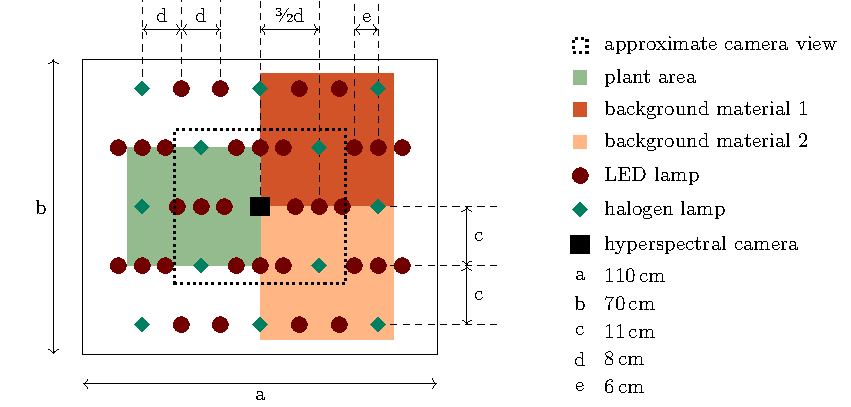
\includegraphics{figures/lamp-layout}
            \caption{Schematic representation of the light and camera arrangement above the plant and background materials.}
            \label{lamp-configuration}
        \end{figure}
        
        A single strawberry leaf was inserted into a transparent leaf chamber of the LI-6400XT photosynthesis system (LI-COR, Lincoln, NE, USA) to acquire gas exchange measurements (transpiration and photosynthesis). The control board also controlled the sampling time steps of the LI-6400XT, using a custom circuit that was connected to the manual sample button on the measurement node. To increase the carbon dioxide concentration in the growth chamber, a constant influx of stabilised air was used. This influx had a carbon dioxide concentration of \SI{500}{ppm} at a rate of \SI{1}{\cubic\metre \per\hour}. For environment sensing at canopy height, we measured the temperature, light intensity and relative humidity. An external probe (Vaisala 50Y, Vaisala, Helsinki, Finland) was used to measure temperature and humidity. The gas exchange device has a PAR probe to measure light intensity. This device was programmed to recreate the temperature measured using the probe inside the chamber, thus preventing the chamber from heating-up due to infrared radiation.
        
        In the centre of the lamp grid, a hyperspectral camera consisting of two camera heads (EP-12, {3D-One}, Sulz, Austria) was placed to monitor the plant. One head is sensitive light in the near-infrared (NIR), while the other is sensitive to the visible range (VIS). We refer to these as H1 and H2, respectively. Both heads capture \SI{12}{\bit} colour information. The sensors were constructed by IMEC (Leuven, Belgium).
        H1 captures light in 25~spectral bands and has a spatial resolution of $403 \times 216$. H2 captures light in 16~spectral bands and has a spatial resolution of $504 \times 270$. A trade-off was made here between spectral accuracy and sampling rate. We set the sampling period to \SI{3}{\second}, which was too fast for using a high-resolution line-scanning sensor. The snapshot camera used here can capture images up to \SI{120}{\hertz}. 
        One spectral filter was used for each sensor to limit the sensitivity range of the visible (VIS) or near-infrared (NIR) spectra. The NIR filter was a long pass filter, starting at \SI{675}{\nano\metre} and cuts-off at \SI{1650}{\nano\metre} (TECHSPEC 675nm 25mm Dia, High Performance Longpass Filter, Edmund Optics, Barrington, NJ, USA), while the VIS filter (SCHOTT BG38, Edmund Optics, Barrington, NJ, USA) starts at \SI{350}{\nano\metre} and cuts-off at \SI{645}{\nano\metre}. This camera does not support an external trigger source, thus the internal trigger source was configured to sample every \SI{3}{\second}. When the responses of the cameras were taken into account, this set-up observed wavelengths in the ranges \SIrange{400}{645}{\nano\metre}, and \SIrange{675}{1000}{\nano\metre} for H1 and H2 respectively. %The detectors are not sensitive to light above \SI{1000}{\nano\metre}. 
        An illustration of the entire set-up is shown in \cref{setup-overview}.
        
        \begin{figure}[thb]
            \centering
            \includegraphics{figures/setup-overview}
            \caption{Experimental set-up inside the growth chamber. The plant (strawberry) was raised to increase the area of the leaf in the images. The sensors (photodiodes, relative humidity and temperature sensor) were mounted at canopy height. The hyperspectral camera was mounted directly above the plant. Twelve halogen lights were mounted at the same height as the camera. A grey PVC plate was used to provide a uniform background.}
            \label{setup-overview}
        \end{figure}
        
        The spectral resolution of H1 varies between \SIlist{6;25}{\nano\metre}, while the spectral resolution of H2 varies between \SIlist{2;14}{\nano\metre}.
        
        A camera always makes an indirect observation, so there might be unwanted interference with the measurements. For instance, the reflective properties of surrounding materials can change, which interferes with the plant measurements. To investigate this, we also included different background materials in the analysis. Four materials were investigated: plywood (hardwood, Van Den Nest, Aalst, Belgium), non-reflective black cotton cloth (Veritas, Kontich, Belgium), grey polyvinyl chloride (PVC) (Scafoam, Scala, Wetteren, Belgium), and Ytong (Xella, Duisburg, Germany). It was not possible to have similar lighting conditions on all four materials simultaneously. Consequently, the experiment was conducted twice. The first experiment used PVC and plywood, while the second used Ytong and cloth. The second experiment was conducted four days after the first one on a different plant. Both plants were grown in the same greenhouse in close proximity, and thus experienced similar conditions before the experiment. Each experiment lasted for \SI{100}{\hour}. Temperature, relative humidity and light radiation were randomly varied, but the same time series was used in both experiments. To generate these random sequences, samples were drawn from a uniform distribution. These distributions ranged between 
        \SIrange{8.8}{32.6}{\celsius} and \SIrange{38.8}{94.6}{\percent} for temperature and relative humidity respectively. These are the set values, which differ from the measured values mentioned above, because the growth chamber was not always able to respond sufficiently fast to the target conditions. The halogen lights were controlled digitally using the DALI interface with brightness vales between 196 (0xC4) and 254 (0xFE) (the maximum value), while the four sets of LED lights were set by sampling a number between 0 and 15, where each bit corresponds to the status of a lamp set. 
        
    \subsection{Data Preparation and Processing}  
        
        The set-up consisted of two independent data sources: the gas exchange system and the hyperspectral camera. They were not synchronised due to the lack of a common trigger source. Hence, the start of measurement was not aligned. This difference was manually corrected by turning on all LED lights at the start of the experiment. Furthermore, the camera did not always sample consistently. As a result, the time points of the images did not always align with those of the gas exchange system. Both the gas exchange and hyperspectral camera systems provide a sample timestamp.  Synchronisation of both sources was achieved using the time points of both sources and linear interpolation to construct sample points on a single time axis.
        
        Time drift between both was negligible for the duration of the experiment because the sample rate was \SI{3}{\second} and the duration of the experiment was only \SI{100}{\hour}. The camera had an internet uplink and was synchronised to a Network Time Protocol (NTP) server. Typical synchronisation offset with NTP-servers are lower than \SI{10}{\milli\second} \citep{marouaniInternal2008}. The LI6400XT has an accurate internal clock that has at most \SI{0.5}{\second} drift after 92~days \citep{li-corinc.Using2012}. Consequently, it is safe to ignore the drift between the two systems.
        
        Photosynthesis is driven to a large extent by light. To maximise the variation in photosynthetic activity of the plant, a substantial range in illumination intensity was applied. Because a camera requires light to operate, the light was never fully turned off. The lowest PAR value that was applied was \SI{70}{\micro\mole \per\square\metre \per\second}, while the highest was \SI{409}{\micro\mole \per\square\metre \per\second}. The camera was set to automatic exposure optimise the dynamic range of each image and reduce over- and underexposed areas. In low illumination conditions, there was a considerable amount of noise. Consequently, after aligning and resampling of the data, the data was further processed using a uniform blur filter of $5\times5$ pixels, to reduce noise in the image. Additionally, the data was rescaled and converted to floating-point to compensate for the variable exposure duration. Details of this transformation are included in the supplementary materials (\cref{st-gain-comp-details}).
        
        The leaves of the strawberry plant displayed limited motion from reorientation, as is evident from  \cref{averaged-image}. Hence, no motion compensation was applied to the image sequence to reduce computational complexity. This also simplified the masking that had to be applied to separate the plant from the background. Each data type has its own mask, which was manually determined and validated. To this end, all images were averaged and a the relevant pixels were selected manually. The validation was performed by generating a video sequence with the mask on top. There are also different masks for the VIS and NIR cameras since they observe the experiment from a different location. Thus, each of the six data types has two masks, one for each camera, resulting in a total of 12~masks.
        
        \begin{figure}[thb]
            \centering
            \includegraphics{figures/averaged-image}
            \caption{Averaged image from every 10th image from the start to the end of the experiment of H1 in the second experiment.}
            \label{averaged-image}
        \end{figure}
        
        Image data are highly correlated, especially for adjacent pixels. Therefore, we constructed two types of datasets. The first dataset averaged over all spatial locations of each mask, to obtain a new data entry. This technique drastically reduced the number of features at each sample point from over \num{10000}\footnote{The number of features is dependent upon the type of data (plant1, plant2, cotton, Ytong, PVC or wood) and the experiment.} to 41. 25 from the NIR camera (H1) and 16 from the VIS camera (H2). We use the following shorthand notation \emph{(25+16)} to denote the number of samples per camera (NIR+VIS). To incorporate spatial effects, a second dataset was constructed using subsampling. The images were spatially sampled randomly without duplicates. When a certain location was considered, all spectral bands were included in the dataset. Subsampling sizes varied between 3 (1+2) and 200 (78+122) for both experiments. The split was designed to have a similar number of features of H1 and H2 at each sample point. Subsampling and averaging also helped to deal with the large amount of data that was captured during the trial. Each image from either H1 or H2 had a size of \SI{4.3}{\mega\byte}, and there were approximately \num{130000} valid data points per trial, resulting in a total dataset size for both trials of slightly more than \SI{2}{\tera\byte}. 
        
        VIs are often used to extract meaningful information from image data, also in hyperspectral imaging \citep{vogelmannRed1993,rouseMonitoring1974,gitelsonSpectral1994,simsRelationships2002,gamonNarrowwaveband1992,behmannDetection2014,jinHyperspectral2016,gaoRecognising2018,alonsoDiurnal2017}. However, only a limited and non-uniformly spaced number of bands are available here, limiting the possibilities to use VIs from literature. Therefore, we generated a custom set of VIs. Based on literature, and taking practical limitations of the number of variables into account, we limited the created VIs to combinations of fractions of band pairs, summarised by \cref{vi1,vi2}. All possible combinations of two spectral bands were generated. \Cref{vi1} is the fraction (F), and \cref{vi2} is the normalised fraction (NF) of a pair of bands. The model automatically selected the relevant indices thanks to regularisation (see below). The spectral bands from H1 were numbered 0~through 24, and those of H2~25 to~40. An index was only included if the absolute value of the maximum value of all Pearson correlation coefficients ($\rho$) with already included indices was lower than 0.95. This boundary ensures that none of the features were (nearly) linearly dependent. Note that the included VIs need not be the same for the different data types since the correlation metric might differ. This technique could generate up to 2459 new features.
        
        
        \begin{equation}
            VI^{F}_{ij} = \dfrac{C_i}{C_j},            \quad i \in\{0,1,\ldots,40\}, j \in \{0,1,\ldots,i-1,i+1,\ldots,40\} \label{vi1}
        \end{equation}
        \begin{equation}
            VI^{NF}_{ij} = \dfrac{C_i - C_j}{C_i+C_j}, \quad i \in\{0,1,\ldots,39\}, j \in \{i+1, i+2, \ldots,40\} \label{vi2}
        \end{equation}
%        \begin{alignat}{2}
%            VI^{F}_{ij} &= \dfrac{C_i}{C_j},            &\quad&i \in\{0,1,\ldots,40\}, j \in \{0,1,\ldots,i-1,i+1,\ldots,40\} \label{vi1} \\
%            VI^{NF}_{ij} &= \dfrac{C_i - C_j}{C_i+C_j}, &&i \in\{0,1,\ldots,39\}, j \in \{i+1, i+2, \ldots,40\} \label{vi2}
%        \end{alignat}
        
        Normally, VIs are only generated on image data from plants, but we also generated them for the background materials to avoid bias due to the generation of possibly more informative features in the comparison between plant- and background-based models.
        
        To assess the variability in performance due to the subsampling in the second dataset, nine independent subsets were constructed of each subsample size. Consequently, partial overlap between datasets was possible.
        
        A linear model combined with Tikhonov (or L2) regularisation \citep{tikhonovSolution1963}, commonly called ridge regression, was used to fit the camera data to the environmental and eco-physiological data. Such a model is well-suited to demonstrate correlations between different datasets and should provide improved prediction performance compared to only using indices \citep{yendrekHighThroughput2017}. It is guaranteed to provide the global optimum and is very fast to fit. This is important since hyperspectral cameras generate vast amounts of data. The Tikhonov regularisation prevents the model to overfit by including the model weights into the optimisation target. 
        The whole pipeline was implemented in Python, with the help of the Pandas \citep{mckinneyData2010,mckinneyPandas2011} and Scikit-Learn \citep{pedregosaScikitlearn2011} libraries and has been open-sourced on GitHub\footnote{\url{https://github.com/opieters/hyperspectral-analysis}}. Part of the dataset is also available with an open-access licence on Zenodo \citep{pieters2020}.
        
        Ridge regression has one hyperparameter that must be optimised. This parameter determines the total magnitude of the model coefficients. As a result, each time series had to be split into three categories: training, validation and test data. The training data was used to train the coefficients of the model, while the validation data was used to select the optimal hyperparameter. The test data was employed to evaluate the performance on unseen data. This latter type of data was not used to optimise the model in any way and thus provided a good indication for the actual performance of the model. To eliminate possible day-night rhythms, the data was split into batches of 3000~samples (\SI{2.5}{\hour}), while 1500~samples (\SI{1.25}{\hour}) between batches were discarded to eliminate the correlation between adjacent batches. This decorrelation was verified after the analysis through an offset between the target and input data (not shown). After selecting the optimal hyperparameter, a final model was trained on both the train and validation data.
        
        \begin{figure}[thb]
            \centering
            \includegraphics{figures/split-visualisation}            
            \caption{Visualisation of the data split in training, validation, and test data for both experiments.}
            \label{data-split}
        \end{figure}
        
        In summary, three different types of linear models were generated based on six different data types. The three model types refer to the kind of input features presented to the model. In the first case, the model was trained on the averaged spectral bands. In the second case, VIs were added to the input feature set. This data-augmentation enabled the model to leverage non-linear dependencies in the data. In the third and final case, the input features consisted entirely of spectral bands, but without averaging over the entire mask. Different materials give rise to distinct data types; plant1, plant2, wood, PVC, Ytong and cotton were the materials considered in this study.
        
    \subsection{Error Metric}
        
        To estimate the modelling capacity of the camera system, different models were created that estimate environmental and eco-physiological data. Comparing the performance of different tasks is crucial. To that end, the normalised mean squared error (NMSE) metric was used:
        
        \begin{equation}
            \text{NMSE} = \ddfrac{\frac{1}{N}\sum_{t=0}^{N-1} (y(t)-\hat{y}(t))^2}{\text{var}(y)} 
        \end{equation}
        
        where $\hat{y}(t)$ is the predicted value from the model, $y(t)$ is the actual value, $\text{var}(\cdot)$ computes the variance and $N$ is the total number of samples considered. This metric has several advantages over a traditional mean squared error comparison. In the first place, it takes the variability of the target signal into account. This eliminates a possible bias towards slow varying signals. Additionally, interpretability is very straightforward. An NMSE of 1.0 corresponds to the mean prediction for all samples, since the numerator reduces to the variance, while an NSME of 0.0 corresponds to a perfect prediction. This property makes it very easy to compare and interpret NMSE values.
        
    \subsection{Variables and Eco-physiological Meaning}  
    
        The gas exchange measurement device (LI6400XT) produced the eco-physiological data to which the hyperspectral image data was fitted. Different environmental and eco-physiological parameters were captured, providing a diverse set of target variables. An overview of the available variables is provided in \cref{parameter-overview}. All variables except for air temperature (\Tair) and relative humidity (\RH) were measured outside the area observed with the camera. This was a requirement due to the high reflectivity of the leaf chamber that resulted in an undesired exposure compensation of the camera. 
        
        \begin{table}[thb]
            \centering
            \caption{Overview of considered environmental and eco-physiological variables.}
            \label{parameter-overview}
            \begin{tabular}{C{2.5cm}L{5cm}C{4cm}C{2.5cm}}
                \toprule
                \textbf{abbreviation} & \textbf{description} & \textbf{unit} & \textbf{sensor}\\
                \midrule
                \arrayrulecolor{black!10!white}
                \Photo & photosynthetic rate & 
                  \si{\micro\mole \of{CO\textsubscript{2}} \per\square\metre \per\second} &
                  LI6400XT \\ 
                \midrule
                \Cond & stomatal conductance & 
                  \si{\mole \of{H\textsubscript{2}O} \per\square\metre \per\second} &
                  LI6400XT \\
                \midrule
                \Transp & transpiration rate & 
                  \si{\milli\mole \of{H\textsubscript{2}O} \per\square\metre \per\second} &
                  LI6400XT \\
                \midrule
                \VPDL & vapour pressure deficit based on leaf temperature & 
                  \si{\kilo\pascal} & LI6400XT\\
                \midrule
                \Tleaf & leaf temperature & \si{\celsius} & LI6400XT \\
                \midrule
                \Tair & {air temperature\newline(growth chamber)} & \si{\celsius} & Vaisala 50Y \\
                \midrule
                \RH & {relative humidity\newline(growth chamber)} & \si{\percent} & Vaisala 50Y\\
                \midrule
                \PAR & {photosynthetically active radiation (growth chamber)} &    
                  \si{\micro\mole\per\square\metre\per\second} & LI6400XT \\
                \arrayrulecolor{black}
                \bottomrule
            \end{tabular}
        \end{table}
   
\section{Results}

    The data were analysed in three steps: first, the environmental conditions were investigated to better understand the eco-physiological responses of the plant in the second and third step. The averaged dataset was augmented with VIs and analysed in the second step, and the subsampled dataset was studied in the third and final step. 

    \subsection{Analysis of the Environmental Conditions}
    
        Normalised density plots of the environmental conditions are depicted in \cref{conditions-plot}. These indicate that \PAR\ vs.\ \RH\ ($\rho = -0.05$) and \PAR\ vs.\ \Tair\  ($\rho = -0.04$) did not show bias towards particular values of either parameter. This is, however, not the case for \RH\ vs.\ \Tair\ ($\rho = -0.27$), due to the inability of the growth chamber to settle at the target point before a new one was set. A combination of low \Tair\ and low \RH\ was not achieved (see \cref{conditions-plot}~(c), lower left corner). High \RH\ values are also less prominent than low ones.
        
        Similar observations were made for the second experiment (not depicted) since the random target sequence was the same for both experiments to simplify the comparison between both extracted datasets. As expected, the main environmental conditions in the growth chamber covered a wide range, but extreme values that cause strong stress conditions were avoided.
    
        \begin{figure}[thb]
            \centering
            \includegraphics{figures/conditions-overview-plot}
            \caption{Normalised density plots of the most important environmental conditions: \PAR, air temperature (\Tair) and relative humidity (\RH) in the growth chamber for the first experiment. The second experiment had similar densities.}
            \label{conditions-plot}
        \end{figure}

    \subsection{Analysis of the Averaged Dataset}
    
        First, we analysed the smaller dataset. This is the dataset that was constructed after averaging over the entire mask, resulting in a single value per spectral band and per mask type. VIs were also generated from the spectral bands. These features were then fitted to target eco-physiological and environmental variables. An overview of the model performance for each data type is depicted in \cref{overview-vi}. Models with VIs are shown using coloured bars, while models without VIs are depicted using a bar with only a blue border.
        
        \begin{figure}[thb]
            \centering
            \includegraphics{figures/grouped-bar-plot-vi}
            \caption{Performance of the linear model for different eco-physiological and environmental parameters. The lower the NMSE, the better. The coloured bars represent models that were trained with raw image data and vegetation indices (VI), while the blue bordered bars are those without VIs.}
            \label{overview-vi}
        \end{figure}
        
        The performance for most photosynthetic rate (\Photo), stomatal conductance (\Cond) and transpiration rate (\Transp) is poor, both with and without VIs. Better performance is observed for \Tleaf\ and to a lesser extent \VPDL. The entire time series of \VPDL\ for plant2 is depicted in \cref{time-plot} for visual inspection. There are several regions where the data fitted very well, but in other parts, there was significant offset from the measured variable, especially at the extremes. Though the model usually follows the correct trend. Visualisations of different tasks for the plant2 time series are depicted in \cref{time-plot}. From this figure, it is clear that models with a high NMSE value have very low extraction efficiency. We consider a fit sufficient if the NMSE value is equal to or below~0.25 for both plant models. 
        
        Eco-physiological tasks with high NMSE values also display major differences in modelling performance between batches of test data (not visualised). This further indicates that the model was unable to extract meaningful information from the spectral features and VIs. The information was either masked by interferers or the camera was unable to capture changes related to these variables. 
        
        \begin{figure}[thb]
            \centering
            \includegraphics{figures/time-plot}
            \caption{Visualisation of the vapour pressure deficit (\VPDL) of plant2 data $y$ and the model prediction $\hat{y}$. The model was trained from the first dataset with vegetation indexes. The different data split types are also indicated. The NMSE values for the train, validation and test data are 0.132, 0.273, and 0.233 respectively.}
            \label{time-plot}
        \end{figure}
        
        For most tasks, there was limited improvement or even reduced performance by adding VIs. Improved performance is strongest for \VPDL, \Tleaf, and \Tair. Reduced performance on the test data can be attributed to overfitting of the model. The performance on the training set has improved, but the models' ability to generalise has decreased, leading to reduced performance. This is especially visible in the case of \RH\ when using Ytong-data. The NMSE value rises from 0.63 to 1.13, above the baseline.   
        
        For all physiological variables, plant1 and plant2 are expected to have better performance than the background materials. However, this is not the case for plant2. While the differences between the plant2 and the background present in the same trial (Ytong and cotton) are low, there is a large difference between plant1 and plant2 for both the average modelling performance of \Photo, \Cond\ and \Transp.  
        
        From the environmental variables, \Tair\ and \PAR\ has the highest extraction precision. \RH\ has a similar NMSE score for all data types except for Ytong. 
        
        
        \begin{table}[thb]
            \centering
            \begin{tabular}{llll}
            \toprule
                       & \textbf{\VPDL} & \textbf{\Tleaf} & \textbf{\Tair} \\
                \textbf{\VPDL}  & 1.0   & 0.89   & 0.76  \\ 
                \textbf{\Tleaf} & 0.89  & 1.0    & 0.92  \\
                \textbf{\Tair}  & 0.76  & 0.92   & 1.0   \\ \bottomrule 
            \end{tabular}
            \caption{Pearson correlation coefficients ($\rho$) of the two well-performing physiological tasks, leaf temperature (\Tleaf) and vapour-pressure deficit (\VPDL), and air temperature (\Tair).}
            \label{physiological-environment-correlation}
        \end{table}
        
\section{Discussion}
    
    The only eco-physiological variables with good performance for both plant time series are \VPDL\ and \Tleaf. However, the background is also good at predicting these. This can be explained by the high correlation between \Tair\ and the variables \VPDL\ and \Tleaf, depicted in \cref{physiological-environment-correlation}. \VPDL\ is driven by relative humidity and leaf temperature, which are in turn affected by air temperature, light intensity and water status \citep{amitranoVapour2019}. The reflection spectrum of plants in the near-infrared region varies when the air temperature changes \citep{carterEffects2000}. These changes are probably detected by the model, leading to good performance of temperature-related variables. The backgrounds considered here might have similar reflective properties. Though their structure cannot change as in the case of plants, they can radiate more or less infrared light, enabling the model to extract the temperature \citep{beltranInfrared1997}.
    
    The results for \Cond\ are in line with previous research by \citet{zarco-tejadaRelationships2013}, who used a similar wavelength range from \SIrange{400}{900}{\nano\metre} and were also unable to extract this parameter. However, others have reported successful extraction of \Cond. \citet{rapaportCombining2015} were able to assess \Cond\ in grapevine, chiefly using the WABI-3 VI. This index uses a spectral band at \SI{1485}{\nano\metre}, which indicates that a wider spectral range is necessary to assess \Cond. Moreover, \citet{rapaportCombining2015} induced a clear treatment. Grapevine leaves were subjected to water-stress, causing stronger changes in \Cond.
    
    The possibility to estimate \Photo\ from hyperspectral data in maize has been reported by \citet{yendrekHighThroughput2017}. They were able to predict the CO\textsubscript{2}-saturated rate of photosynthesis ($V_\text{max}$) from hyperspectral imaging and a partial least squares (PLS) regression model. They indicated important peak wavelengths at \SI{554}{\nano\metre} and \SI{719}{\nano\metre}. Though the VIS and NIR cameras have nearby bands at \SI{552}{\nano\metre} and \SI{724}{\nano\metre}, there are fewer bands available compared to the study by \citet{yendrekHighThroughput2017}, which acquired the spectral reflection of maize at a resolution of \SI{1}{\nano\metre}. While their results are significant for $V_\text{max}$, the results are probably insufficient to capture the subtle dynamics of the study presented in this paper. Due to the two treatments that were applied in the study by \citet{yendrekHighThroughput2017}, low nitrogen availability and elevated ozone concentrations, $V_\text{max}$ varied from approximately \SIrange{7}{62}{\micro\mole\per\square\metre\per\second}, while \Photo\ only varies from \SIrange{3.1}{14.7}{\micro\mole\per\square\metre\per\second}. Furthermore, their model also has a root mean square error (RMSE) score of 6.6, resulting in low predictive performance for the range of the current study, and thus also has limited applicability to monitor small changes of \Photo.
    
    As mentioned in the introduction, SIF is a promising indicator of photosynthetic activity. It originates from initial reactions in Photosystem II and I, which have narrow peaks around \SI{690}{\nano\metre} and \SI{760}{\nano\metre} respectively. Resolving these peaks requires high spectral resolution ($\le\SI{5}{\nano\metre}$), which is not possible with the technology used in this study \citep{bandopadhyayReview2020}. A snapshot camera with improved resolution should be able to compute SIF and thus be able to better assess photosynthetic activity.
    
    Unlike the current study, \citet{wekslerHyperspectralPhysiological2020} were able to measure \Transp\ with hyperspectral imagery in young pepper plants. They used a selection of spectral bands at \SIlist{523;697;818}{\nano\metre} with high spectral resolution using as VIS-NIR camera (\SIrange{400}{1000}{\nano\metre}). Unlike most studies, the study by \citet{wekslerHyperspectralPhysiological2020} also characterised momentary transpiration. The major difference between the method from their study to the current one, is the plant age. In this study, mature plants were used, unlike the rapidly growing plants in their experiment. Moreover, they measured transpiration using a balance, not with a gas exchange system. 
    
    From these studies, we identified four causes that might explain the poor results for \Cond, \Photo, and \Transp. First, the spectral range was insufficient. More specifically, higher wavelengths up to at least \SI{1500}{\nano\metre} are needed to assess these properties based on literature. Second, the spectral resolution needs to increase to preferably \SI{1}{\nano\metre}, and the band spacing should be more uniform. Third, other studies which investigated eco-physiological properties applied clear treatments \citep{zhaoNitrogen2005,zarco-tejadaSpatiotemporal2013,behmannDetection2014,silva-perezHyperspectral2018}. These cause more pronounced spectral and eco-physiological changes. Therefore, estimation is more direct and less prone to disturbances that mask eco-physiological changes. Fourth, the plant species and age also have an effect on the plant dynamics, where young plants are expected to have stronger variation.
    
    Additionally, a camera is a sensor \emph{at a distance}, meaning that there is no direct contact with the imaged object. This has both positive and negative consequences. The main positive effect is limited to no interference with the object and rapid capture of large amounts of data. However, this creates a disadvantage also due to the distance between object and sensor. There might be interfering materials present that can distort the measurement. For instance, the transmittance of the air layer between the camera and the sample can change depending on environmental changes. Similarly, the reflective properties of materials present in the growth chamber can also change as a result of variable environmental conditions. These changes are also picked up by the camera and can distort the measurement. Usually, such changes are negligible, but when very subtle variability in the plant is under investigation, they might become important.  Moreover, it is difficult to compensate for these possible effects during the analysis.
    
    Both \PAR\ and \Tair\ are well assessed for plants and all backgrounds. The good performance of \PAR\ is expected since the camera directly observes light and can reconstruct the spectrum used in the measurement of \PAR. As mentioned before, spectral changes due to temperature can explain the good modelling performance of \Tair. It was verified that the camera's responses are not significantly temperature-dependent other than increased white noise at elevated temperatures (data not presented).
    
    The poor NMSE value of \RH\ from the data is in stark contrast to the other environmental variables.  A possible reason why these have a high NMSE value is, that there is no infrared radiation around \SI{2}{\micro\metre} captured by the camera nor emitted by the lights. Consequently, none of the strong absorption peaks of water was captured.
    
    %Adding VIs to the dataset did not offer significant improvements to most variables. As such, the mechanistic basis of VIs was not investigated. The exhaustive use of VIs can be a good first step towards the discovery of new physiological VIs. 
    The inclusion of VIs does not improve the results much. Consequently, it is not relevant to investigate each of these indices separately and relate them to physiological processes occurring in the plant. If there would have been a significant improvement by including these empirically created indices, additional analysis and experiments would be needed to identify which indices are the most explanatory and explain why these were found. For instance, the generalisation from one plant to another should be tested by using at least three plants: one for training, one for validation and one for testing. 
    

\section{Conclusion}
    
    The experimental study presented in this manuscript investigated the accessibility of gas exchange variables of plants from hyperspectral image data. The novelty of this study is that these parameters were investigated without the presence of strong biotic or abiotic stress factors with high temporal resolution (\SI{3}{\second}) over the duration of one week. This setup is relevant to monitor the dynamics of plants' physiological responses. Increasingly, researchers are investigating the dynamic behaviour of plants as these are crucial in determining plant productivity in continuously fluctuating environments such as those in agricultural fields.
    
    The analysis indicated that the information content of the hyperspectral data is low for \Photo, \Cond, and \Transp. A possible explanation is the limited variability due to the much lower treatment effect and low-resolution spectral sensing capabilities. The lack of a clear stress-inducing treatment causes less variation of the eco-physiological variables observed. Induced variations were possibly not significant enough to be detectable among other interfering and noise signals that are present in the image data. Additionally, the spectral resolution and range were limited. Plant species and age can also have an effect on performance.  \VPDL\ and \Tleaf\ are good performing eco-physiological tasks. Environmental variables also show varying results. As expected, PAR is well assessed, as is \Tair. \RH\ cannot be extracted due to the lack of wavelengths above \SI{2}{\micro\metre}. We suspect that the reflection spectrum changes depending on temperature, which enables the model to accurately predict \Tair. \Tleaf\ and \VPDL\ are strongly correlated to \Tair\ might explain why these eco-physiological parameters could be assessed.
    
    Current snapshot hyperspectral technologies are not yet well suited to monitor the dynamic responses of plants. Major improvements upon sensitivity and spectral resolution are probably required to enable the detection of subtle changes of eco-physiological parameters in stress-free conditions.
    
    \FloatBarrier

    \bibliographystyle{elsarticle-harv}
    \bibliography{bibliography}


\section{Author contributions statement (CRediT)}

    % https://www.elsevier.com/authors/journal-authors/policies-and-ethics/credit-author-statement
    
    \noindent
    \begin{tabularx}{\linewidth}{@{}lX}
    Olivier Pieters & Conceptualization, Methodology, Data curation, Software, Validation, Investigation, Writing - original draft, Writing - review \& editing, Visualization\\
    Tom De Swaef & Conceptualization, Methodology, Writing - original draft, Writing - review \& editing\\
    Peter Lootens & Conceptualization, Methodology, Writing - review \& editing\\
    Michiel Stock & Conceptualization, Methodology, Writing - review \& editing\\
    Isabel Rold\'an-Ruiz & Conceptualization, Methodology, Writing - review \& editing\\
    Francis wyffels & Conceptualization, Methodology, Writing - review \& editing\\
    \end{tabularx}

\section{Conflicts of Interest}
    
    The authors declare no conflict of interest.
    
    \FloatBarrier

\section{Supplementary Materials}

    \subsection{Shutter time and Gain Compensation Details}\label{st-gain-comp-details}
        
        The shutter time and gain values are automatically determined by the camera to achieve higher dynamic range, especially in low-light conditions. Consequently, the resulting image data have to be rescaled to the same scale. This is done using the following transformation:
        
        \begin{equation}
            q = \dfrac{p}{r_c (s - x_0) + y_0} \label{camera-correction-eq}
        \end{equation}
        
        Where $q$ is the transformed version of pixel value $p$, with shutter time $s$. The other values depend upon the camera used and gain setting. The values are listed in \cref{camera-correction}. These were obtained by maintaining the same light intensity, while varying and camera configuration. Transforming these using \cref{camera-correction-eq}, results in a constant value.
    
\end{document}
